\section{The Web as a platform}

\subsection{From OS to Web platform}

The focus of the software industry switched from native desktop applications to mobile and web applications.
In this 

\subsection{The languages of the web}

Python(1993), Javascript(1995), Ruby(1993), PHP(1995) and Java(1994) were all created around the same time, in the early 90's.
Java imposes itself early as the language of the web, and never really decreased. It is a solid, professional language used by most of the industry.
But it is too big, and too slow growing for the exact same reason.

Python is older (1991), and was always seen as a general purpose language.
It is only in 2003, with the Django framworks that Python start to be seen as a web language.

PHP short-lived as the easy-to-use scripting language, it is now backed by facebook, but is on the decline.

Ruby took-off in 2005 with Rails, and is still in active use.
But it seems it is going to be eclipsed by Javascript.

Since a few years, Javascript is in a constant rise as the main language of the web, because of Ajax first, and then Node.js
What is so different with Javascript ?
It is omnipresent, from every browser, to the server.
And it is a target for LLVM.
Because of this position, it became fast (V8, ASM.js ...) and usable (ES6, ES7).

\subsection{Explosion of Javascript popularity}

\subsubsection{In the beginning}

Javascript was created by Brendan Eich at Netscape around May 1995, and released to the public in September.
The initial name of the project was Mocha, then LiveScript, the name Javascript was finally adopted to leverage the trend around Java.
The latter was considered the hot new web programming language at this time.
It was quickly adopted as the main language for web servers, and everybody was betting on pushing Java to the client as well.
The history proved them wrong.
% Javascript slowly took over the client, and is now pushing toward the server.
% But that was not a calm and linear journey.

In 1995, when Javascript was released, the world wide web started its wide adoption.\ftnt{http://www.internetlivestats.com/internet-users/}
Browsers were emerging, and started a battle to show off the best features and user experience to attract the wider public.\footnote{to get an idea of the web in 1997 : \url{http://1x-upon.com/}}
Microsoft released their browser Internet Explorer 3 in June 1996 with a concurrent implementation of Javascript.
They changed the name to JScript, to avoid trademark conflict with Oracle Corporation, who owns the name Javascript.
The differences between the two implementations made difficult for a script to be compatible to both.
At the time, signs started to appear on web pages to warn the user about the ideal web browser to use for the best experience on this page.
This competition was fragmenting the web.
% and the overall user experience could be improved by /// according the technology ///.

To stop this fragmentation, Netscape submitted Javascript to Ecma International for standardization in November 1996.
In June 1997, ECMA International released ECMA-262, the first specification of ECMAScript, the standard for Javascript.
A standard to which all browser should refer for their implementations.
% TODO more on the Ecma specification ?

The base for this specification was designed in a rush. The version released in 1995 was finished within 10 days.
Because of this precipitation, the language has often been considered poorly designed and unattractive.
Moreover, Javascript was intended to be simple enough to attract unexperienced developers, by opposition to Java or C++, which targeted professional developers.
For these reasons, Javascript started with a poor reputation among the developer community.

But things evolved drastically since.
When a language is released, available freely at a world wide scale, and simple enough to be handled by a generation of teenager inspired by the technology hype, it produce an effervescent community around what is now one of the most popular and widely used programming language.

\subsubsection{Rising of the unpopular language}

Javascript started as a programming language to implement short interactions on web pages.
The best usage example was to validate some forms on the client before sending the request to the server.
This situation hugely improved since the beginning of the language.
So much that web-based, Javascript applications are currently now favored instead of rich, native desktop applications.

ECMA International released several version in the few years following the creation of Javascript.
The first and second version, released in 1997 and 1998, brought minor revisions to the initial draft.
However, the third version, released in the late 1999, contributed to give Javascript a more complete and solid foundation as a programming language.
From this point on, the consideration for Javascript keep improving.

An important reason for this reconsideration started in 2005.
James Jesse Garrett released \textit{Ajax: A New Approach to Web Applications}, a white paper coining the term Ajax \cite{Garrett2005}.
This paper point the trend in using this technique, and explain the consequences on user experience.
Ajax stands for Asynchronous Javascript And XML.
It consists of using Javascript to dynamically request and refresh the content of a web page.
The advantage is that it avoids to request a full page from the server.
Javascript is not anymore confined to the realm of small user interactions on a terminal, it can be proactive and responsible for a bigger part in the system spanning from the server to the client.
Indeed, this ability to react instantly to the user started to narrow the gap between web and native applications.
%, while keeping all the advantages of web-based applications.
At the time, the first web applications to use Ajax were Gmail, and Google maps\footnote{A more in-depth analysis of the history of Ajax, given by late Aaron Swartz \url{http://www.aaronsw.com/weblog/ajaxhistory}}.

Around this time, the Javascript community started to emerge.
The third version of ECMAScript had been released, and the support for Javascript was somewhat homogeneous on the browsers but far from perfect.
Moreover, Javascript is only a small piece in the architecture of a web-based client application.
The DOM, and the \texttt{XMLHttpRequest} method, two components on which AJAX relies, still present heterogeneous interfaces among browsers.
To leverage the latent capabilities of Ajax, and more generally of the web, Javascript framework were released with the goal to straighten the differences between browsers implementations.
Prototype\ftnt{http://prototypejs.org/} and DOJO\ftnt{https://dojotoolkit.org/} are early famous examples, and later jQuery\ftnt{https://jquery.com/} and underscore\ftnt{http://underscorejs.org/}.
These frameworks are responsible in great part to the wide success of Javascript and of the web technologies.

In the meantime, in 2004, the Web Hypertext Application Technology Working Group\ftnt{https://whatwg.org/} formed to work on the fifth version of the HTML standard.
This new version provide new capabilities to web browsers, and a better integration with the native environment.
It features geolocation, file API, web storage, canvas drawing element, audio and video capabilities, drag and drop, browser history manipulation, and many mores
It gave Javascript the missing pieces to become a true language for developing rich application.
The first public draft of HTML 5 was released in 2008, and the fifth version of ECMAScript was released in 2009.
With these two releases, ECMAScript 5 and HTML5, it is a next step toward the consideration of Web-based technologies as equally capable, if not more, than native rich applications on the desktop.
Javascript became the programming language of this rising application platform.

However, if web applications are overwhelmingly adopted for the desktop, HTML5 is not yet widely accepted as ready to build complete application on mobile, where performance and design are crucial.
Indeed web-technologies are often not as capable, and well integrated as native technologies.
But even for native development, Javascript seems to be a language of choice.
An example is the React Native Framework\ftnt{https://facebook.github.io/react-native/} from Facebook, which allow to use Javascript to develop native mobile applications.
They prone the philosophy \textit{"learn once, write anywhere"}, in opposition to the usual slogan \textit{"write once, run everywhere"}.\footnote{Used firstly by Sun for Java, but then stolen by many others}
% Another example is Gnome-shell. It uses Javascript to build its interface, and extensions.
% PhoneGap (Cordova) is a huge effort toward bringing web technologies to the mobile. 

\subsubsection{Current situation}

\cit{When JavaScript was first introduced, I dismissed it as being not worth my attention. Much later, I took another look at it and discovered that hidden in the browser was an excellent programming language.}{Douglas Crockford}

% \cit{JavaScript is the world's most ubiquitous computing runtime.}{John Lam}

The success of Javascript is due to many factors ; I mentioned previously the standardization, Ajax libraries and HTML5.
Another factor, maybe the most important, is the View Source menu that reveals the complete source code of any web application.
\textit{The view source menu is the ultimate form of open source}\ftnt{http://blog.codinghorror.com/the-power-of-view-source/}.
It is the vector of the quick dissemination of source code to the community, which picks, emphasizes and reproduces the best techniques.
This brought open source and collaborative development before github. \comment{TODO neither open source nor collaborative development are the correct terms}
Moreover, all modern web browsers now include a Javascript interpreter, making Javascript the most ubiquitous runtime in history \cite{Flanagan2006}.
% Every browser include development tools for Javascript, making it the most ubiquitous development environment, as well.

When a language like Javascript is distributed freely with the tools to reproduce and experiment on every piece of code.
When this distribution is carried during the expansion of the largest communication network in history.
Then an entire generation seizes this opportunity to incrementally build and share the best tools they can.
This collaboration is the reason for the popularity of Javascript on the Web.

% I want to say that Javascript took off because it was carried by the open source community.
% The goal is to introduce the following facts : JS is widely used in the open source community.
% I need to find the argument saying that open source is taking over closed sources : Javascript / open source is taking over Java / closed source.

% TO READ :
% http://www.javaworld.com/article/2077224/learn-java/is-javascript-here-to-stay-.html
% http://blog.codinghorror.com/the-power-of-view-source/
% http://blog.codinghorror.com/javascript-the-lingua-franca-of-the-web/
% http://shaver.off.net/diary/2007/05/10/the-high-cost-of-some-free-tools/


% This success is obvious on the web and in the open source communities.
It seems to also infiltrate many other fields of IT, but it is hard to give an accurate picture of the situation.
There is no right metrics to measure programming language popularity.
In the following paragraphs, I report some popular metrics and indexes available on the net.
More detailed informations are available section \ref{appendix:langpop}.

\paragraph{Search engines}

The TIOBE Programming Community index is a monthly indicator of the popularity of programming languages.
It uses the number of results on many search engines as a measure of the activity of a programming language.
Javascript ranks 6th on this index, as of April 2015, and it was the most rising language in 2014.
However, the measure used by the TIOBE is controversial.
Some says that the measure is not representative.
It is a lagging indicator, and the number of pages doesn't represent the number of readers.

On the other hand, the PYPL index is based on Google trends to measure the activity of a programming language.
Javascript ranks 7th on this index, as of May 2015.

From these indexes, the major programming languages are Java, C/C++ and C\#.
The three languages are still the most widely taught, and used to write softwares.
But Javascript is rising to become one of these important languages.

\paragraph{Developers collaboration platforms}

Github is the most important collaborative development platform, with around 9 millions users.
Javascript is the most used language on github since mid-2011, with more than 320 000 repositories.
The second language is Java with more than 220 000 repositories.

\comment{TODO : graph of Github repositories by languages}

StackOverflow, is the most important Q\&A platform for developers.
It is a good representation of the activity around a language.
Javascript is the second language showing the most activity on StackOverflow, with more than 840 000 questions.
The first one is Java with more than 850 000 questions.

Black Duck knowledgebase analyzes 1 million repositories over various forges, and collaborative platforms to produce an index of the usage of programming language in open source communities.
Javascript ranks second.
C is first, and C++ third.
Along with Java, the four first languages represent about 80\% of all programming language usage.

% TODO redo this graph, it is ugly.
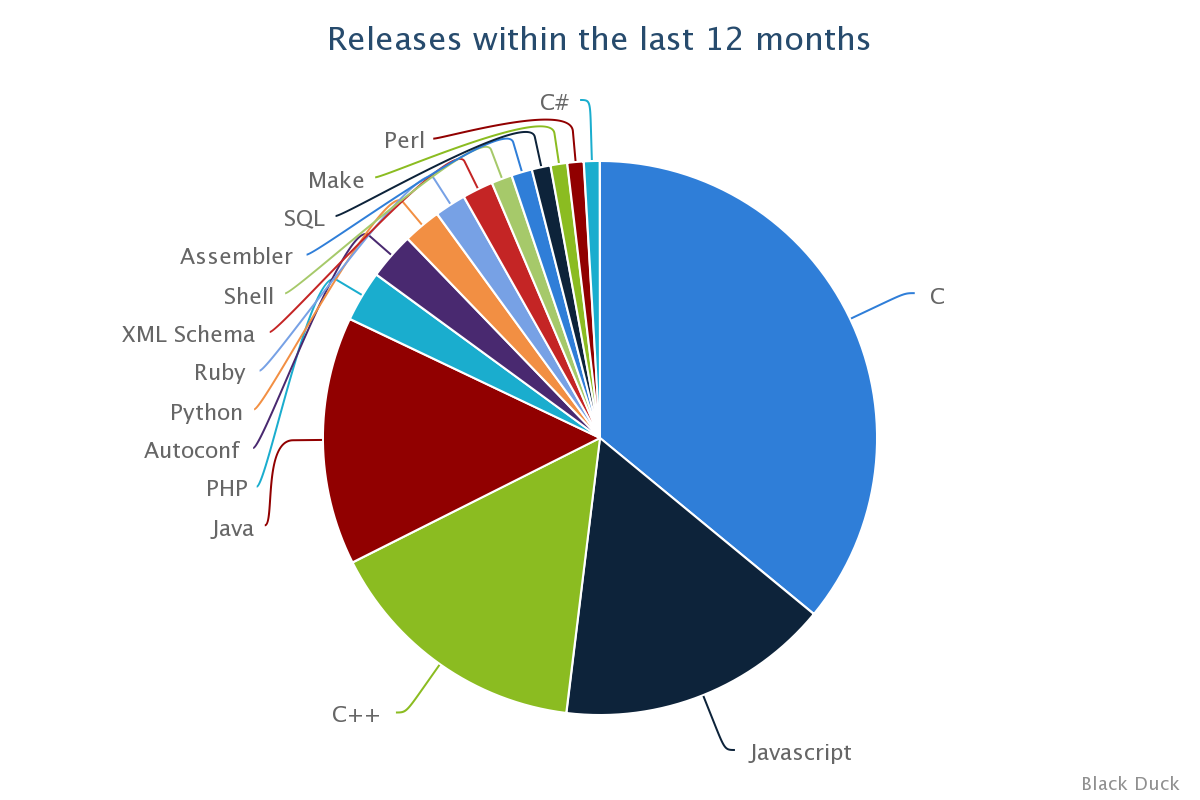
\includegraphics[width=0.9\linewidth]{../../data/js-trends/black-duck-15}

\paragraph{Jobs}

All these metrics are representing the visible activity about programming language.
But not the entire software industry is open source, and the activity is rather opaque.
To get a hint on the popularity of programming languages used in the software industry, let's look at the job offerings.
Indeed provide some insightful trends.
Javascript developers ranked at the third position, right after SQL developers and Java developers.
Then come C\# and C developers.

% TODO redo this graph, it is ugly.
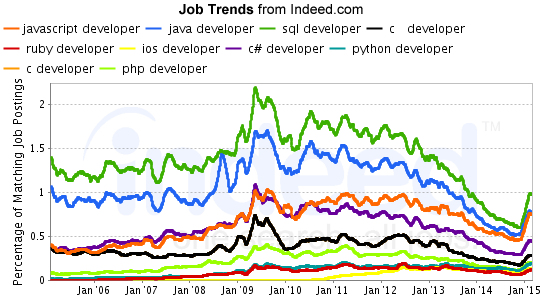
\includegraphics[width=0.9\linewidth]{../../data/js-trends/jobgraph}

All these metrics represent different faces of the current situation of Javascript adoption.
We can safely say that Javascript is one of most important language of this decade, along with Java, C/C++.
It is widely used in open source projects, and everywhere on the web.
But it is also trending, and maybe slowly replacing languages like Java.
% TODO continue this

\paragraph{Future trends}

\comment{TODO}

Code reuse.
Why it never worked ?




\comment{em-scripten}

https://github.com/kripken/emscripten
Javascript is a target language for LLVM, therefor everything can compile to Javascript : JS is the assembler of the web.

\comment{Isomorphic Javascript}

Server-side Javascript

https://www.meteor.com/
https://facebook.github.io/flux/
Javascript can be executed both on the client and the server.
That allow use-cases never possible before (server pre-rendering, same team ...)

\comment{Reactive}

http://facebook.github.io/react/
Javascript is used to model the flow of propagation of state in a web application



---

Some facts to include :
https://www.destroyallsoftware.com/talks/the-birth-and-death-of-javascript
The Atom editor is written in Javascript node.js.
Now, major PaaS (which one) support node.js by default.
Heroku support Python, Java, Ruby, Node.js, PHP, Clojure and Scala
Amazon Lambda Web service support node.js in priority.
npm raises 8m.
http://techcrunch.com/2015/04/14/popular-javascript-package-manager-npm-raises-8m-launches-private-modules/

% >>> I want to say that Javascript is now broadly used.
% Let's just look at the numbers : Javascript is the most popular language on Github, and npm has more package than any other package manager.
% Javascript has the more broadly deployed runtime.
% ... and so on
% >>> the conclusion is : Javascript is now a major language, and it is more than worth the consideration we are giving it in this PhD thesis.

With numbers from Worldline about Java and Javascript usages.

It ends with some success stories with Javascript (Paypal, Linkedin and so on ...).

-> There is a growing mass of developers for Javascript.
And even for those who don't program in Javascript, there is transpilers.
Javascript is here to stay : http://www.javaworld.com/article/2077224/learn-java/is-javascript-here-to-stay-.html (an article from 1996, where Java was still the hot new language)
